\documentclass[conference]{IEEEtran}
\IEEEoverridecommandlockouts
\usepackage{cite}
\usepackage{amsmath,amssymb}
\usepackage{graphicx}
\usepackage{booktabs}

% \setcounter{dbltopnumber}{3}
% \renewcommand{\dbltopfraction}{0.95}

% Generated by generate_figures.py; do not edit by hand.
% TSCS result macros are dimensionless sigma/(4L) ratios.
% BackendMaxDiff is an absolute difference in sigma/(4L).
% FirstOrderCutoff is the dimensionless kL threshold pi*P.
\newcommand{\ConvErrorNFiveTwelve}{\ensuremath{2.81142\times 10^{-5}}}
\newcommand{\FlatTSCSRatioTwenty}{\ensuremath{0.9999612}}
\newcommand{\BackendMaxDiff}{\ensuremath{1.59298\times 10^{-5}}}
\newcommand{\AmpTSCSFlat}{\ensuremath{0.9999612}}
\newcommand{\AmpTSCSFive}{\ensuremath{0.9948396}}
\newcommand{\AmpTSCSTen}{\ensuremath{0.9926829}}
\newcommand{\FreqTSCSTwelve}{\ensuremath{1.010974}}
\newcommand{\FreqTSCSSixteen}{\ensuremath{0.9968797}}
\newcommand{\FreqTSCSTwenty}{\ensuremath{0.9926829}}
\newcommand{\FirstOrderCutoff}{\ensuremath{15.70796}}
\newcommand{\FlatOrderDoublingMaxChange}{\ensuremath{5.03819\times 10^{-6}}}
\newcommand{\ProductionMaxTSCSChange}{\ensuremath{7.53315\times 10^{-6}}}
\newcommand{\ProductionMaxPatternChange}{\ensuremath{2.30664\times 10^{-5}}}
\newcommand{\MARCorrugatedMaxTSCSChange}{\ensuremath{2.42789\times 10^{-6}}}
\newcommand{\MARCorrugatedMaxPatternChange}{\ensuremath{7.644\times 10^{-6}}}
\newcommand{\MARCorrugatedMaxResidual}{\ensuremath{9.65836\times 10^{-7}}}
\newcommand{\MARModeDoublingTSCSChange}{\ensuremath{3.3308\times 10^{-16}}}
\newcommand{\MARModeDoublingPatternChange}{\ensuremath{6.25461\times 10^{-16}}}
\newcommand{\MARProjectionDoublingTSCSChange}{\ensuremath{2.96379\times 10^{-11}}}
\newcommand{\MARProjectionDoublingPatternChange}{\ensuremath{8.26557\times 10^{-8}}}
\newcommand{\MARProjectionDoubledResidual}{\ensuremath{3.04278\times 10^{-8}}}


\begin{document}

\title{E-Polarized Plane-Wave Scattering by a Finite 
Sinusoidal PEC Grating via the Nystr\"om Method%
\thanks{This work was supported by the National Research 
Foundation of Ukraine via project \#2025.07/0094.}}

\author{\IEEEauthorblockN{A. Petryshyn, S.V. Dukhopelnykov, and T.L. Zinenko}
\IEEEauthorblockA{\textit{O. Y. Usikov Institute for Radiophysics and Electronics of the}\\
\textit{National Academy of Sciences of Ukraine}\\
Kharkiv 61085, Ukraine}}

\maketitle

\begin{abstract}
This paper presents a Nystr\"om treatment for two-dimensional (2D) E-polarized
plane-wave scattering by a finite sinusoidal grating made of a perfect electric
conductor (PEC). The inverse-square-root endpoint singularity of the induced current
is extracted as a factor, and the logarithmic integral equation is
differentiated before the resulting Cauchy-singular equation is discretized at
Gauss--Chebyshev nodes. The formulation accommodates arbitrary incidence
angles. Convergence under interpolation order increment and agreement with independently
implemented analytical-regularization and pulse-basis methods are demonstrated
for a flat strip, whose total scattering cross section approaches the
geometrical-optics limit at high frequency. Results for a symmetric five-period
grating show how corrugation height and electrical size shape the
absolute far-field scattering pattern. Above the first
propagating-harmonic threshold, broadened finite-grating lobes appear near the
reference directions of the corresponding infinite grating, while finite-length
effects preserve the specular reflection lobe and end-generated background. The
study therefore clarifies how infinite-grating Floquet harmonics propagation directions can be used to
interpret scattering by finite gratings.
\end{abstract}

\begin{IEEEkeywords}
Electromagnetic scattering, sinusoidal open strip, integral equations, Nystr\"om
method, perfect electric conductors.
\end{IEEEkeywords}

\section{Introduction}

Finite corrugated conductors combine periodic-surface physics with end effects
that are absent from an infinite grating.  Even a scalar two-dimensional model
therefore has to resolve a singular edge current, interaction across several
corrugations, and radiation into both halfspaces.  Early numerical treatments
of two-dimensional diffraction and the associated quadrature techniques are
surveyed by Nazarchuk~\cite{nazarchuk1989}.  Differentiated formulations based
on the method of discrete singularities (MDS) and the Nystr\"om method for open
perfect-electric-conductor (PEC) arcs, including interpolation quadratures and
supplementary conditions, were developed in
\cite{nosich2005,nosich2007,nosich_josa2007,gandel2010}.  Related
edge-conditioned and exponentially convergent Nystr\"om schemes for open
structures are reported in~\cite{tong2006,tsalamengas2006,shapoval2011}.
Accurate regularized analyses of curved open PEC reflectors provide further
full-wave benchmarks~\cite{oguzer2001,oguzer2009}.

The scattering by PEC finite sinusoidal grating has also been studied with other
methods.  Kobayashi and Eizawa used a Wiener--Hopf technique analysis for the 
E-polarization case~\cite{kobayashi1991} and H-polarized analysis was reported
in~\cite{eizawa2014}.  Vinogradova, Kobayashi, and Eizawa later developed a
full-wave E-polarized solution by the analytical regularization~\cite{vinogradova2019}.
Related resonant configurations formed by two finite sinusoidal gratings were
analyzed in~\cite{vinogradova2021}.  These studies emphasize that the angles of radition
of the Floquet harmonics remain useful references, but a grating with only a few periods
does not possess exact Floquet channels.

This paper presents a compact Nystr\"om solution for the electric-field integral equation 
(IE) established in the scattering by a finite sinusoidal PEC grating - see Fig. 1.  Its 
contributions are threefold.  First, the grating geometry is assumed symmetric,
all size parameters are referred to the half-span $L$, and the incidence angle
is arbitrary.  Second, the solution accuracy is assessed by an
$L^2$-norm convergence study and a triple comparison with other methods.  Third,
the polar scattering patterns and the total scattering cross section (TSCS) reveal 
the effects of corrugation height and electrical size for a five-period grating.

\section{Formulation and Nystr\"om Discretization}
\label{sec:method}

\subsection{Geometry and Boundary-Value Problem}

For a structure invariant along $z$, E polarization is represented by the
scalar electric field component $U=E_z$ in the $x$--$y$ plane.  The scatterer is a
zero-thickness PEC strip, whose cross-section $\Gamma$ is symmetric in $x$ and parameterized as
\begin{equation}
 \boldsymbol \Gamma(t)=\bigl(Lt,\;h\cos(\pi Pt)\bigr),
 \qquad -1\leq t\leq 1,
 \label{eq:geometry}
\end{equation}
where $2L$ is its projected width, $h/L$ is the relative corrugation height,
and the integer $P$ is the number of complete periods.  Its projected period
is $\Lambda=2L/P$.  Hence geometry is specified by $h/L$ and $P$, while
frequency enters only through the electric size $kL$.  The notation and
angle convention are summarized in Fig.~\ref{fig:geometry}.

\begin{figure}[!t]
 \centering
 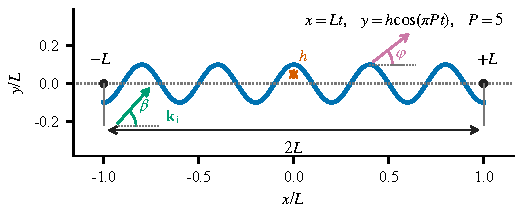
\includegraphics[width=\columnwidth]{fig1_geometry.pdf}
 \caption{Symmetric finite sinusoidal PEC grating and angle convention.  The
 incident wave vector is $\boldsymbol{k}_{\rm i}=k\widehat{\boldsymbol d}$,
 where $\widehat{\boldsymbol d}=(\cos\beta,\sin\beta)$; observation angle
 $\varphi$ is measured counterclockwise from $+x$.}
 \label{fig:geometry}
\end{figure}

With the suppressed time factor $e^{-i\omega t}$, a unit-amplitude incident
plane wave is
\begin{equation}
 U^{\rm inc}(\boldsymbol r)
 =\exp\!\left(ik\widehat{\boldsymbol d}\mathbin{\cdot}\boldsymbol r\right),
 \qquad
 \widehat{\boldsymbol d}=(\cos\beta,\sin\beta).
 \label{eq:incident}
\end{equation}

Thus constant-phase fronts travel along $\widehat{\boldsymbol d}$.  In computaions, we
use normal incidence, $\beta=\pi/2$; no such restriction is made in the
equations.  The scattered field $U^{\rm sc}$ has to satisfy the Helmholtz equation,
the outgoing Sommerfeld condition, local power finiteness at both endpoints,
and the Dirichlet boundary condition
\begin{equation}
 U^{\rm inc}+U^{\rm sc}=0 \quad \text{on }\Gamma .
 \label{eq:pec}
\end{equation}

\subsection{Log-Singular Integral Equation}

The scattered field can be presented as a convolution of the surface current
density $q$ with the Green's function (single-layer representation).  As its 
endpoint behavior is known from the local 
power density finiteness condition, this density is factored as
\begin{equation}
 q(t)|\boldsymbol r'(t)|
 =\frac{v(t)}{\pi\sqrt{1-t^2}},
 \label{eq:edgefactor}
\end{equation}
where $v$ is smooth.  Equation~\eqref{eq:edgefactor} extracts the singular
factor; it does not remove the physical edge singularity.  Define
$R(t,\tau)=|\boldsymbol r(t)-\boldsymbol r(\tau)|$,
$G(s)=H_0^{(1)}(ks)$, $w(t)=(1-t^2)^{-1/2}$, and
$u_0(\tau)=U^{\rm inc}(\boldsymbol r(\tau))$.  Then, the boundary condition (3)
yields the following logarithmically singular IE
\begin{equation}
 \frac{1}{\pi}\int_{-1}^{1}G(R(t,\tau))v(t)w(t)\,dt=-u_0(\tau).
 \label{eq:ie}
\end{equation}

Following the Nystr\"om treatments for open PEC arcs
in~\cite{nosich2005,nosich2007,gandel2010}, the logarithmically singular
IE~\eqref{eq:ie} is differentiated with respect to $\tau$, producing a
Cauchy-singular IE.  In particular, let
\begin{align}
 c_H&=-\frac{2i}{\pi},                                                   \label{eq:ch}\\
 K(t,\tau)&=\frac{\partial}{\partial\tau}
 H_0^{(1)}\!\left(kR(t,\tau)\right)-\frac{c_H}{t-\tau},                 \label{eq:kernel}\\
 f(\tau)&=-\frac{d}{d\tau}U^{\rm inc}(\boldsymbol r(\tau))
 =-ikU^{\rm inc}(\boldsymbol r(\tau))
 \widehat{\boldsymbol d}\mathbin{\cdot}\boldsymbol r'(\tau).
 \label{eq:rhs}
\end{align}

The Cauchy-part extraction follows the normalized formulations
in~\cite{nosich2005,nosich2007}.  The
small-argument expansion of $H_0^{(1)}$ in~\cite{shapoval2011} gives
$c_H=-2i/\pi$; consequently, $K$ is a continuous function.  The
differentiated equation is
\begin{equation}
 \frac{1}{\pi}\operatorname{p.v.}\!\int_{-1}^{1}
 \left[\frac{c_H}{t-\tau}+K(t,\tau)\right]
 \frac{v(t)}{\sqrt{1-t^2}}\,dt=f(\tau).
 \label{eq:cauchyie}
\end{equation}

Further, we discretize the Cauchy-singular equation (1) using the interpolation 
quadratures described in~\cite{nosich2005,nosich2007,nosich_josa2007}, with first-kind
Gauss--Chebyshev nodes and interlaced second-kind collocation points
\begin{align}
 t_i&=\cos\frac{(2i-1)\pi}{2N},&&i=1,\ldots,N, \notag\\
 \tau_j&=\cos\frac{j\pi}{N},&&j=1,\ldots,N-1.                    \label{eq:nodes}
\end{align}

Denoting the density samples by $v_i=v(t_i)$, we obtain the following
boundary rows for $j=1,\ldots,N-1$:
\begin{equation}
 \frac{1}{N}\sum_{i=1}^{N}
 \left[\frac{c_H}{t_i-\tau_j}+K(t_i,\tau_j)\right]v_i=f(\tau_j).
 \label{eq:nystrom}
\end{equation}

Here, the Gauss--Chebyshev weight $\pi/N$ combines with the factor $1/\pi$
in~\eqref{eq:cauchyie}, yielding the factor $1/N$.

As in~\cite{nosich2005,nosich2007}, a weighted supplementary condition restores
the integration constant lost upon differentiation and hence equivalence
to~\eqref{eq:ie},
\begin{equation}
 \frac{1}{N}\sum_{i=1}^{N}M(t_i)v_i=c,                                  \label{eq:supprow}
\end{equation}
where
\begin{align}
 M(t)&=\int_{-1}^{1}H_0^{(1)}\!\left(kR(t,\tau)\right)
          \frac{d\tau}{\sqrt{1-\tau^2}},                                \label{eq:mdef}\\
 c&=-\int_{-1}^{1}U^{\rm inc}(\boldsymbol r(\tau))
          \frac{d\tau}{\sqrt{1-\tau^2}}.                               \label{eq:cdef}
\end{align}

The logarithmic self term in $M$ is subtracted analytically and its smooth
remainder is evaluated by a higher-order Chebyshev rule.  Equations
\eqref{eq:nystrom} and~\eqref{eq:supprow} form an $N\times N$ dense system.

\subsection{Far Field and TSCS}

For $\widehat{\boldsymbol s}(\varphi)=(\cos\varphi,\sin\varphi)$, we define
the far-field scattering pattern $\Phi_{\rm sc}$ by
$U^{\rm sc}(r,\varphi)\sim e^{ikr}\Phi_{\rm sc}(\varphi)/\sqrt{kr}$.
Then, the single-layer far-field asymptotics and the same quadrature
in~\cite{nosich2007} give
\begin{equation}
 \Phi_{\rm sc}^{(N)}(\varphi)
 =\sqrt{\frac{2}{\pi i}}\,\frac{1}{N}\sum_{i=1}^{N}
 e^{-ik\widehat{\boldsymbol s}(\varphi)\cdot\boldsymbol r(t_i)}v_i.
 \label{eq:farfield}
\end{equation}

For the unit incident amplitude, the total scattering cross section is
\begin{equation}
 \sigma=\frac{1}{k}\int_{0}^{2\pi}|\Phi_{\rm sc}(\varphi)|^2\,d\varphi.
 \label{eq:tscs}
\end{equation}

It has the required length dimension.  The polar plots below display the
associated angular scattering pattern
 $10\log_{10}[|\Phi_{\rm sc}(\varphi)|^2/(kL)]$; they are not normalized to the
 maximum of each curve.

The verification, representative field pattern, height sweep, and
electrical-size sweep are presented in Figs.~\ref{fig:verification}--
\ref{fig:frequency}, respectively.

% IEEEtran cannot place a double-column float on the page where it is defined.
% Declare the result figures before the next page so they remain in numerical
% order and are placed before the bibliography rather than interrupting it.
\begin{figure*}[!t]
 \centering
 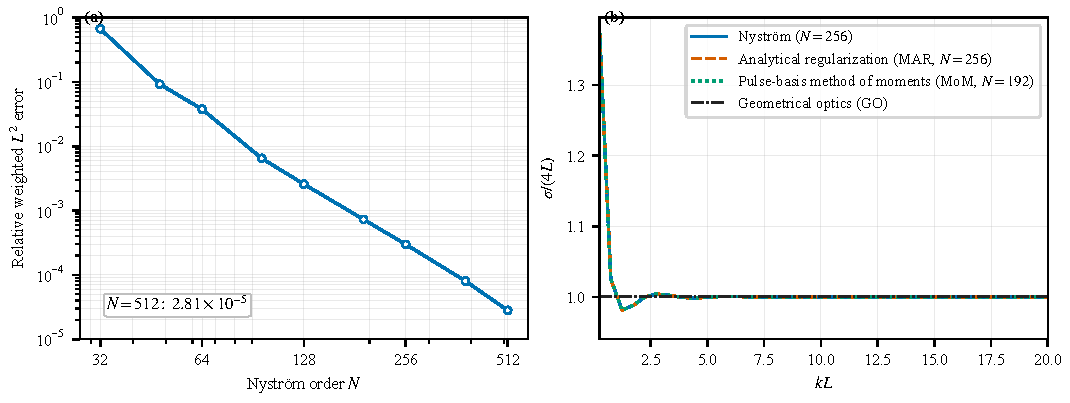
\includegraphics[width=\textwidth]{fig2_verification.pdf}
 \caption{Verification. (a) Relative $L^2$ error of the smooth density versus
 interpolation order for $P=5$, $h/L=0.10$, and $kL=20$.
 (b) Flat-strip total scattering cross section (TSCS), normalized by its
 geometrical-optics limit $4L$, from the differentiated Nystr\"om method
 ($N=256$), the method of analytical regularization [[xxx]] (MAR; $N=256$), and a
 pulse-basis method of moments [[yyy]](MoM; 192 elements); the dash-dotted line is the
 geometrical-optics (GO) limit.}
 \label{fig:verification}
\end{figure*}

\begin{figure*}[!t]
 \centering
 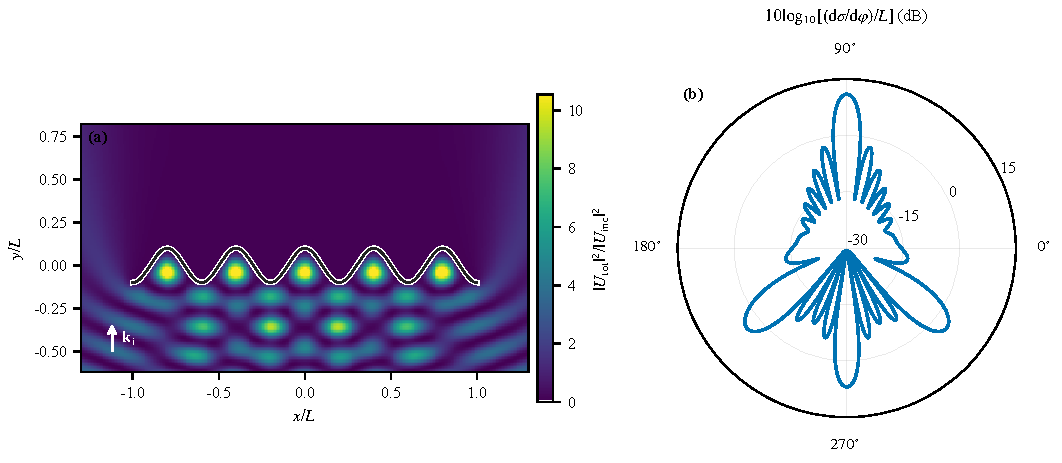
\includegraphics[width=\textwidth]{fig3_field_pattern.pdf}
 \caption{Five-period grating at $P=5$, $h/L=0.10$, $kL=20$, and
 $\beta=\pi/2$. (a) Relative total-field intensity
 $|U^{\rm inc}+U^{\rm sc}|^2/|U^{\rm inc}|^2$. (b) Absolute polar scattering
 diagram based on $\Phi_{\rm sc}$ in~\eqref{eq:farfield}, shown as
 $10\log_{10}[|\Phi_{\rm sc}(\varphi)|^2/(kL)]$ on the common $-30$ to $+15$
 dB scale.}
 \label{fig:fieldpattern}
\end{figure*}

\begin{figure*}[!t]
 \centering
 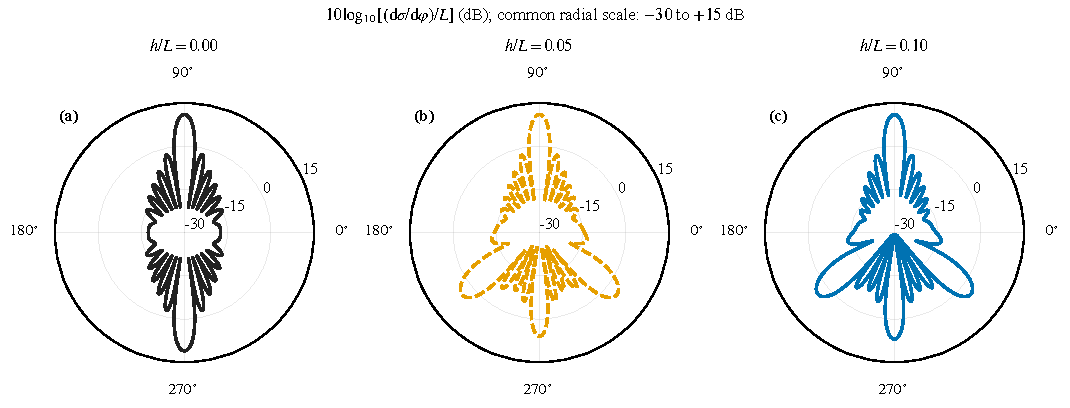
\includegraphics[width=\textwidth]{fig4_amplitude_polar.pdf}
 \caption{Absolute polar scattering diagrams based on $\Phi_{\rm sc}$
 in~\eqref{eq:farfield}, shown as
 $10\log_{10}[|\Phi_{\rm sc}(\varphi)|^2/(kL)]$, for $P=5$, $kL=20$, and
 $\beta=\pi/2$: (a) $h/L=0$; (b) $h/L=0.05$; and (c) $h/L=0.10$. Each panel
 contains one curve and uses the common $-30$ to $+15$ dB scale.}
 \label{fig:amplitude}
\end{figure*}

\begin{figure*}[!t]
 \centering
 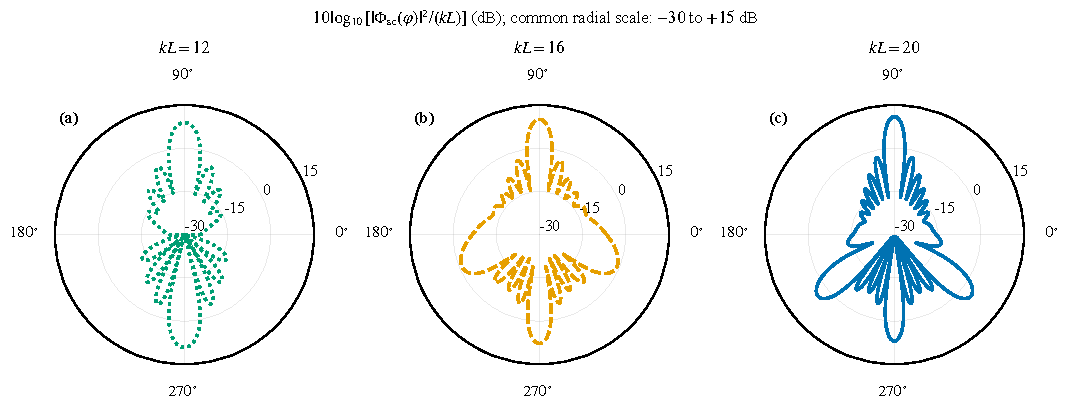
\includegraphics[width=\textwidth]{fig5_frequency_polar.pdf}
 \caption{Absolute polar scattering diagrams based on $\Phi_{\rm sc}$
 in~\eqref{eq:farfield}, shown as
 $10\log_{10}[|\Phi_{\rm sc}(\varphi)|^2/(kL)]$, for $P=5$, $h/L=0.10$, and
 $\beta=\pi/2$: (a) $kL=12$; (b) $kL=16$; and (c) $kL=20$. Each panel
 contains one curve and uses the common $-30$ to $+15$ dB scale. The
 first-order periodic-reference harmonics are cut off at $kL=5\pi$ and
 propagate above it.}
 \label{fig:frequency}
\end{figure*}

For reference, it is instructive to keep in mind the plane-wave
scattering by the similar infinite sinusoidal PEC grating. In this case,
the scattered field is expandable in terms of the Floquet series, where 
the harmonics have the wavenumbers 
\begin{equation}
 \xi_m=\cos\beta+\frac{m\pi P}{kL},\qquad |\xi_m|<1.                    \label{eq:floquet}
\end{equation}

Their upper- and lower-halfspace angles are $\arccos\xi_m$ and
$2\pi-\arccos\xi_m$, respectively.  In our case ofthe finite grating,
these angles are only the markers for the broad lobes of the scattering 
pattern; below they are called infinite-grating
reference directions.  At the normal incidence, this reduces to
\begin{equation}
 \cos\varphi_m=\frac{m\pi P}{kL},\qquad
 \left|\frac{m\pi P}{kL}\right|<1.                                    \label{eq:floquetnormal}
\end{equation}

For instance, if $P$=5, the first-order harmonics become propagating at
\begin{equation}
 kL=\pi P=\FirstOrderCutoff \quad (P=5).                                 \label{eq:cutoff}
\end{equation}

\section{Numerical Results}
\label{sec:results}

\subsection{Convergence and Cross-Validation}

Fig.~\ref{fig:verification}(a) reports a relative weighted $L^2$ error of
the smooth part of the current density for $P=5$, $h/L=0.10$, $kL=20$, and $\beta=\pi/2$.  Let
$I_Nv_N$ denote its Chebyshev interpolant and set
$\theta_\ell=(\ell+1/2)\pi/4096$.  With the $N_{\rm ref}=800$ solution as the
reference, the plotted error is
\begin{equation}
 \epsilon_N=\left[
 \frac{\sum_{\ell=0}^{4095}|I_Nv_N(\cos\theta_\ell)
       -I_{800}v_{800}(\cos\theta_\ell)|^2}
      {\sum_{\ell=0}^{4095}|I_{800}v_{800}(\cos\theta_\ell)|^2}
 \right]^{1/2}.
 \label{eq:l2error}
\end{equation}

This midpoint sampling in $\theta$ approximates the
$L^2_{1/\sqrt{1-t^2}}$ norm in $t$.  For
$N=32,48,64,96,128,192,256,384,512$, the error decreases systematically and
reaches \ConvErrorNFiveTwelve at $N=512$.  The latter order is used for all
corrugated-grating results below.  Repeating every unique publication case at
$N=800$ changes the TSCS by at most \ProductionMaxTSCSChange and the full
complex far-field pattern by at most \ProductionMaxPatternChange in relative
$L^2$ norm.

The second test uses a flat strip ($h=0$) with electrical siz varying in the range
$0.25\leq kL\leq20$.  Fig.~\ref{fig:verification}(b) compares the present
Nystr\"om implementation with separately obtained results of the
analytical-regularization and pulse-basis method-of-moments treatments.  The
maximum spread in $\sigma/(4L)$ among the three results is \BackendMaxDiff.
The first two use $N=256$, and the pulse discretization uses 192 elements.
In the most demanding scenario, at $kL=20$, doubling those orders changes the
TSCS by at most \FlatOrderDoublingMaxChange.
At $kL=20$ the Nystr\"om value is
\FlatTSCSRatioTwenty.  This is close to the geometrical-optics limit
$\sigma/(4L)\to1$ for a broadside-illuminated flat PEC strip of projected
width $2L$~\cite{shapoval2011}, but it is correctly retained as a
finite-frequency value.

\subsection{Representative Five-Period Grating}

Fig.~\ref{fig:fieldpattern} shows the results for the normal incidence for
$P=5$, $h/L=0.10$, and $kL=20$.  As visible on panel (a), below the grating the 
incident and reflected fields interfere and form the standing wave pattern; above it, 
the pattern reveals the shadow.  The polar scattering pattern on panel (b) gives 
$\Phi_{\rm sc}$ in~\eqref{eq:farfield} over $0\leq\varphi<2\pi$.  At this
electric size, the $m=\pm1$ periodic-reference Floquet
harmonics are propagating, and the calculated finite-grating pattern contains
broad off-normal lobes near the corresponding reference directions, in the 
reflection half-space. Despite sinusoidal corrugation, the specular
reflection lobe and the edge-generated background remain because only five
periods are retained.

% Coarsely equalize the two columns on the final page, as recommended by
% IEEEtran for camera-ready conference papers.
\enlargethispage{-1.25in}
\subsection{Height and Electric-Size Dependence}

At fixed $P=5$ and $kL=20$, increasing $h/L$ changes the phase and magnitude
of the induced current across each corrugation.  Fig.~\ref{fig:amplitude}
shows the resulting power redistribution among the specular and off-normal lobes.
Because every panel has the same absolute radial scale, changes in level can be
compared directly.  The corresponding normalized TSCS values, together with
those for the electrical-size sweep below, are listed in
Table~\ref{tab:tscs_sweeps}.

\begin{table}[!t]
 \caption{Normalized TSCS for the height and electrical-size sweeps in
 Figs.~\ref{fig:amplitude} and~\ref{fig:frequency} ($P=5$, $\beta=\pi/2$).}
 \label{tab:tscs_sweeps}
 \centering
 \setlength{\tabcolsep}{3.5pt}
 \begin{tabular}{cc@{\quad}cc}
  \toprule
  \multicolumn{2}{c}{$kL=20$} & \multicolumn{2}{c}{$h/L=0.10$} \\
  \cmidrule(r){1-2}\cmidrule(l){3-4}
  $h/L$ & $\sigma/(4L)$ & $kL$ & $\sigma/(4L)$ \\
  \midrule
  $0$    & \AmpTSCSFlat & $12$ & \FreqTSCSTwelve \\
  $0.05$ & \AmpTSCSFive & $16$ & \FreqTSCSSixteen \\
  $0.10$ & \AmpTSCSTen  & $20$ & \FreqTSCSTwenty \\
  \bottomrule
 \end{tabular}
\end{table}

The variation in frequency changes both the overall electric width and the set of
propagating periodic-reference Floquet harmonics.  The three cases for $P=5$ and
$h/L=0.10$ in Fig.~\ref{fig:frequency} are also tabulated in
Table~\ref{tab:tscs_sweeps}.
At $kL=12$ the first-order periodic harmonics are evanescent.  They become
propagating above the threshold ~\eqref{eq:cutoff}, so the first-order
finite-grating lobes appear only in the $kL=16$ pattern and scan further from
the grazing directions at $kL=20$.  Their widths can be expected to get narrower if 
the number of periods $P$ is taken larger.

\section{Conclusion}

A log-singular integral equation, discretized with the Nystr\"om
technique, has been studied for the E-polarized plane-wave scattering by a
finite zero-thickness sinusoidal PEC grating.  We have visualized the solution 
convergence in the $L2$-norm and demonstrated the agreement with two other 
computational techniques, one of which (MAR) also has mathematically guaranteed 
convergence. Additionally, we have demonstrated that the frequency dependence of  
the broadside-illuminated flat PEC strip TSCS, computed with our code, tends to 
the geometrical-optics limit $4L$ and coinsides with results of ~\cite{shapoval2011}
The operating frequency and the grating period determine when the periodic-reference 
Floquet harmonics become propagating, while the grating electric size (number of periods)
and the corrugation height mainly influence the width and intensity of the
grating lobes.

\begin{thebibliography}{00}

\bibitem{nazarchuk1989}
Z.~T. Nazarchuk, \emph{Numerical Investigation of Wave Diffraction from
Cylindrical Structures}. Kyiv, Ukraine: Naukova Dumka, 1989, in Russian.

\bibitem{nosich2005}
A.~A. Nosich and Yu.~V. Gandel, ``Method of discrete singularities in the
accurate modeling of a reflector beam waveguide,'' in \emph{2005 IEEE MTT-S
Int. Microwave Symp. Dig.}, Long Beach, 2005, pp. 1083--1086,
doi: 10.1109/MWSYM.2005.1516860.

\bibitem{nosich2007}
A.~A. Nosich and Yu.~V. Gandel, ``Numerical analysis of quasioptical
multireflector antennas in 2-D with the method of discrete singularities:
E-wave case,'' \emph{IEEE Trans. Antennas Propag.}, vol. 55, no. 2,
pp. 399--406, Feb. 2007, doi: 10.1109/TAP.2006.889811.

\bibitem{nosich_josa2007}
A.~A. Nosich, Yu.~V. Gandel, T.~Magath, and A.~Altintas, ``Numerical analysis
and synthesis of 2D quasi-optical reflectors and beam waveguides based on an
integral-equation approach with Nystr\"om's discretization,'' \emph{J. Opt.
Soc. Amer. A}, vol. 24, no. 9, pp. 2831--2836, Sep. 2007,
doi: 10.1364/JOSAA.24.002831.

\bibitem{gandel2010}
Yu.~V. Gandel, ``Boundary-value problems for the Helmholtz equation and their
discrete mathematical models,'' \emph{J. Math. Sci.}, vol. 171, no. 1,
pp. 74--88, 2010, doi: 10.1007/s10958-010-0127-3.

\bibitem{tong2006}
M.~S. Tong and W.~C. Chew, ``Nystr\"om method with edge condition for
electromagnetic scattering by 2D open structures,'' \emph{Prog. Electromagn.
Res.}, vol. 62, pp. 49--68, 2006, doi: 10.2528/PIER06021901.

\bibitem{tsalamengas2006}
J.~L. Tsalamengas, ``Exponentially converging Nystr\"om's methods for systems
of singular integral equations with applications to open/closed strip- or
slot-loaded 2-D structures,'' \emph{IEEE Trans. Antennas Propag.}, vol. 54,
no. 5, pp. 1549--1558, May 2006, doi: 10.1109/TAP.2006.874348.

\bibitem{shapoval2011}
O.~V. Shapoval, R. Sauleau, and A.~I. Nosich, ``Scattering and absorption of
waves by flat material strips analyzed using generalized boundary conditions
and Nystr\"om-type algorithm,'' \emph{IEEE Trans. Antennas Propag.}, vol. 59,
no. 9, pp. 3339--3346, Sep. 2011, doi: 10.1109/TAP.2011.2161547.

\bibitem{oguzer2001}
T. O\u{g}uzer, A.~I. Nosich, and A. Alt\i nta\c{s}, ``E-polarized beam
scattering by an open cylindrical PEC strip having an arbitrary
``conical-section'' profile,'' \emph{Microw. Opt. Technol. Lett.}, vol. 31,
no. 6, pp. 480--484, Dec. 2001, doi: 10.1002/mop.10067.

\bibitem{oguzer2009}
T. O\u{g}uzer, A. Alt\i nta\c{s}, and A.~I. Nosich, ``Integral equation analysis 
of an arbitrary-profile and varying-resistivity cylindrical reflector illuminated 
by an E-polarized complex-source-point beam,'' \emph{J. Opt. Soc. America A}, 
vol. 26, no. 7, pp. 1525--1532, 2009, doi: 10.1364/JOSAA.26.001525.

\bibitem{kobayashi1991}
K. Kobayashi and T. Eizawa, ``Plane wave diffraction by a finite sinusoidal
grating,'' \emph{IEICE Trans. Electron.}, vol. E74-C, no. 9, pp. 2815--2826,
Sep. 1991, doi: 10.1587/e74-c\_9\_2815.

\bibitem{eizawa2014}
T. Eizawa and K. Kobayashi, ``Wiener--Hopf analysis of the H-polarized plane
wave diffraction by a finite sinusoidal grating,'' \emph{Prog.
Electromagn. Res.}, vol. 149, pp. 1--13, 2014,
doi: 10.2528/PIER14063007.

% Balance the references below the two full-width figures on the final page.
% \newpage
\bibitem{vinogradova2019}
E.~D. Vinogradova, K. Kobayashi, and T. Eizawa, ``Full wave analysis of plane
wave diffraction by a finite sinusoidal grating: E-polarization case,''
\emph{Wave Motion}, vol. 86, pp. 44--62, Mar. 2019,
doi: 10.1016/j.wavemoti.2018.12.006.

\bibitem{vinogradova2021}
E.~D. Vinogradova and K. Kobayashi, ``Complex eigenvalues of natural
TM-oscillations in an open resonator formed by two sinusoidally corrugated
metallic strips,'' \emph{IET Microw., Antennas Propag.}, vol. 15, no. 10,
pp. 1283--1298, 2021, doi: 10.1049/mia2.12166.

\end{thebibliography}

\end{document}
